%%==================================================
%% chapter04.tex for TJU Master Thesis
%% Encoding: UTF-8
%%==================================================

\chapter{基于频移目标函数的反射全波形反演}

论文第三章提出的$Q$-RWI框架是基于数据残差的最小二乘目标函数来实现的,该目标泛函
对于理论的合成数据有很理想的效果,那是因为在合成数据实验中我们假设已知了模型
速度的高波数成分和低波数成分,即振幅的残差只由$Q$不准引起。
在实际勘探地震数据处理中,要获取低波数的速度模型相对可行,高波数的速度
模型很难精确获取,而高波数的速度成分又是影响地震波振幅的最大因素。此外,
地震波振幅还受数据采集环境的影响,如环境噪音、检波器与地表耦合情况等。
引起振幅残差的成因的不确定性给第三章提出的基于数据残差最小的$Q$-RWI法造成了致命
的影响。

如何孤立地将地震衰减对地震数据的影响从数据中提取出来是$Q$-RWI法走向实用的关键。
本章将从地震数据属性出发,寻找只与$Q$相关的地震数据属性,
并将其应用到$Q$-RWI中。


\vspace{0.5cm}
\section{引言}
\begin{figure*}[!htbp]
    \centering
    \subfigure[]{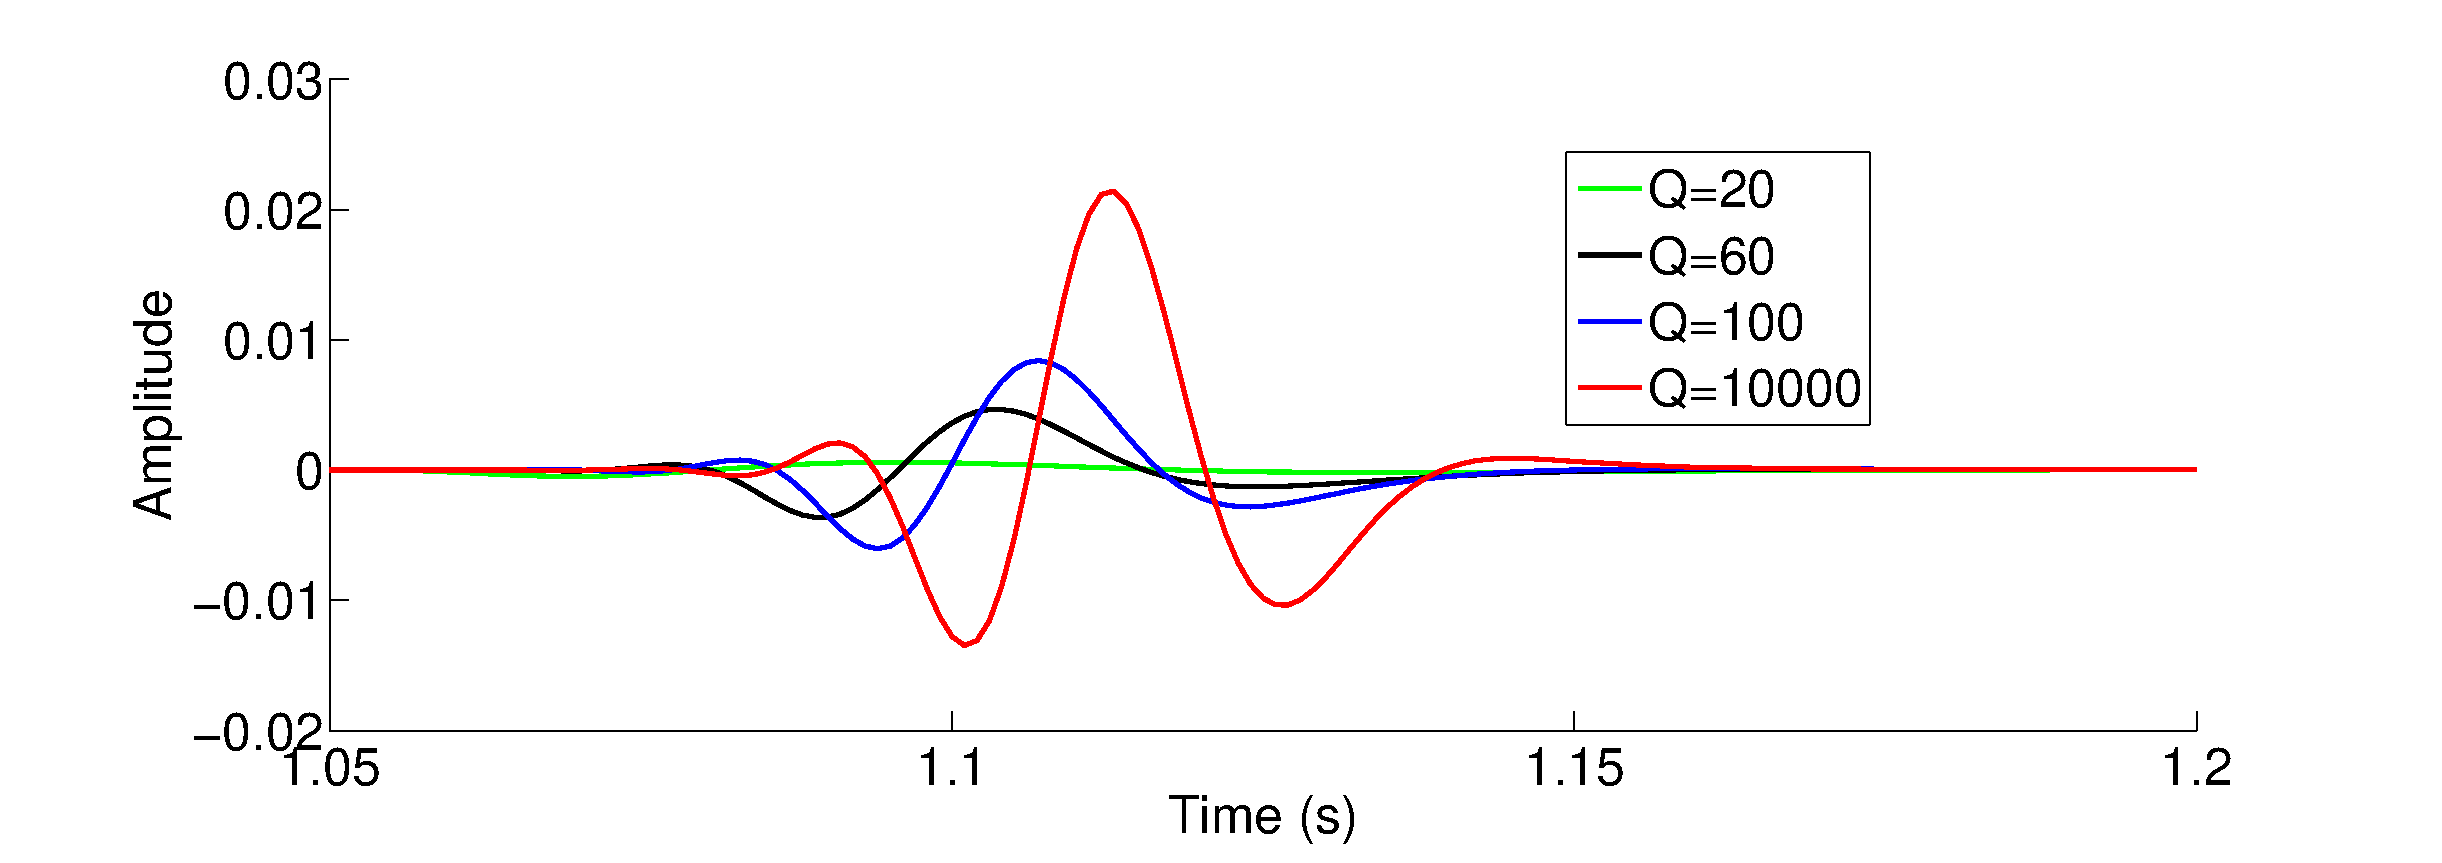
\includegraphics[width=0.92\linewidth]{figure/wavelet}}
    \subfigure[]{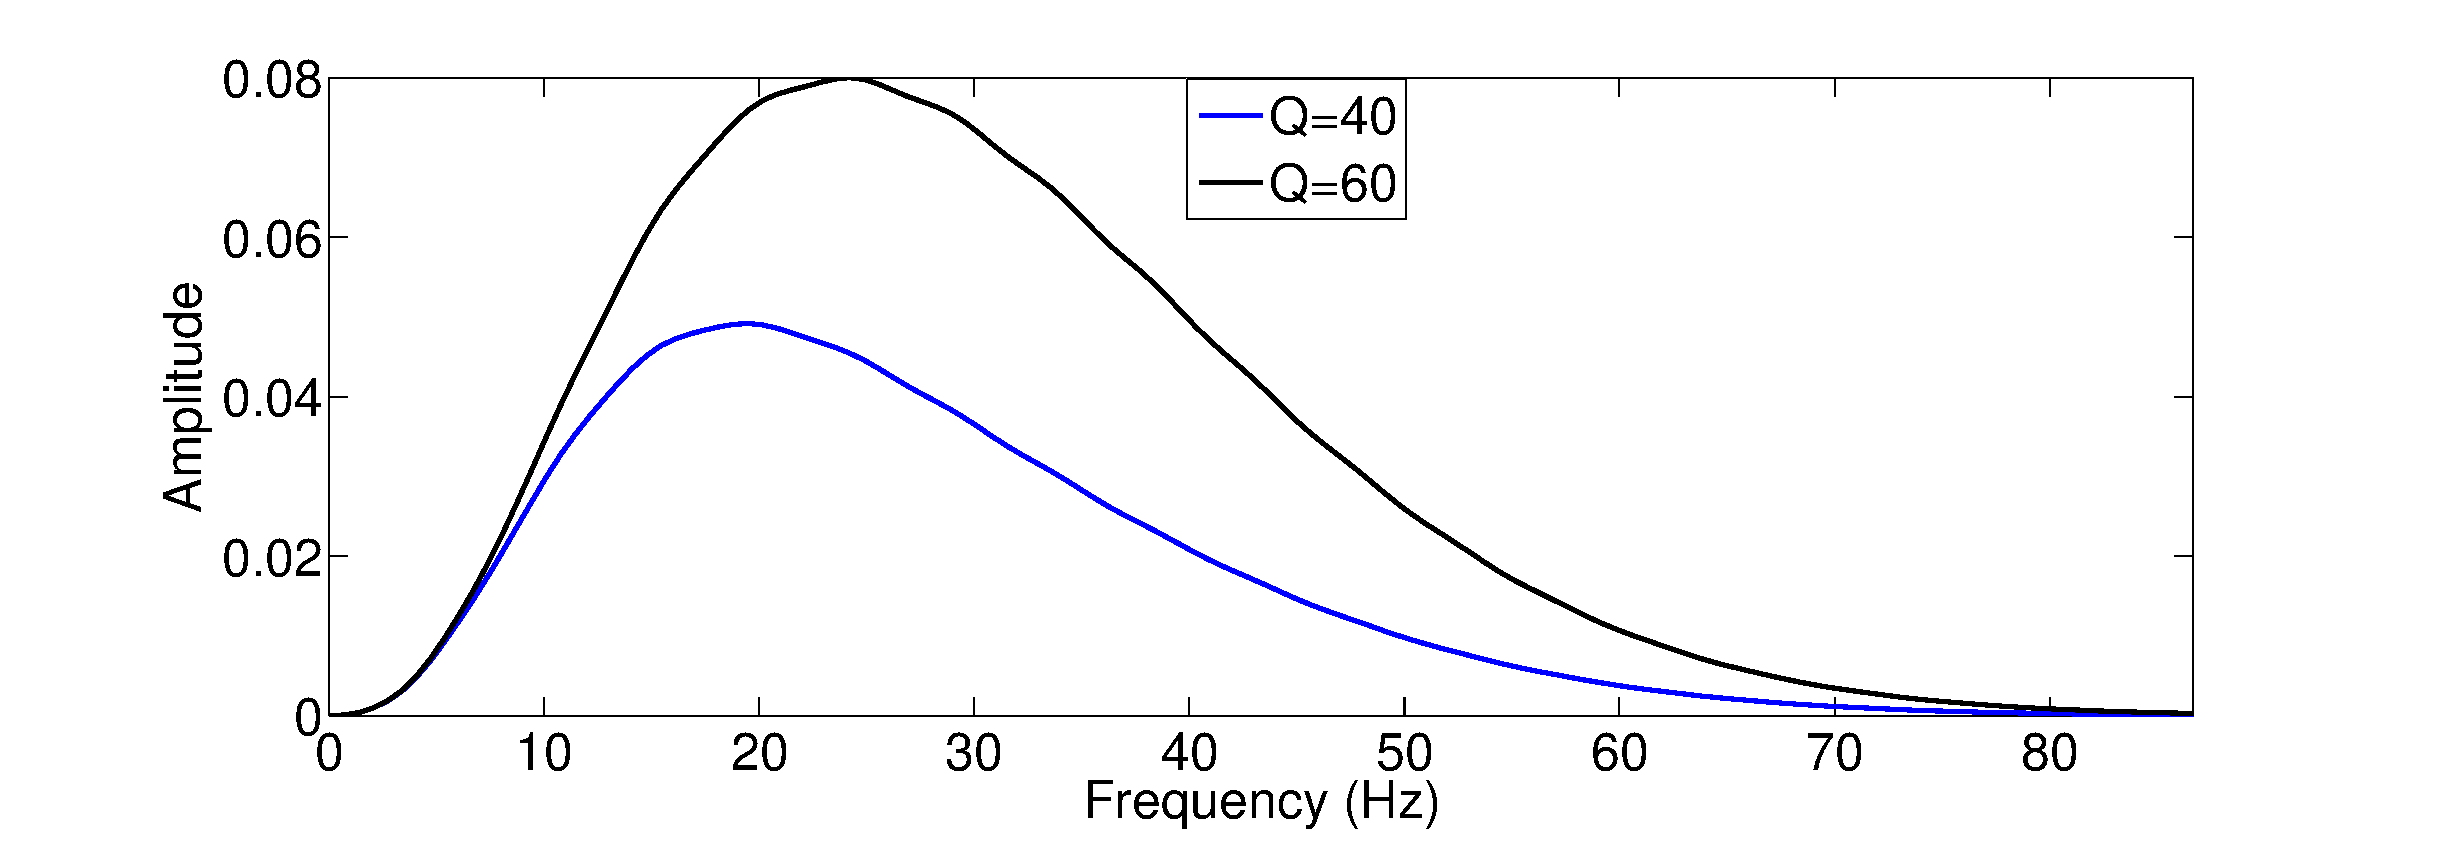
\includegraphics[width=0.92\linewidth]{figure/spectrum}}
    \subfigure[]{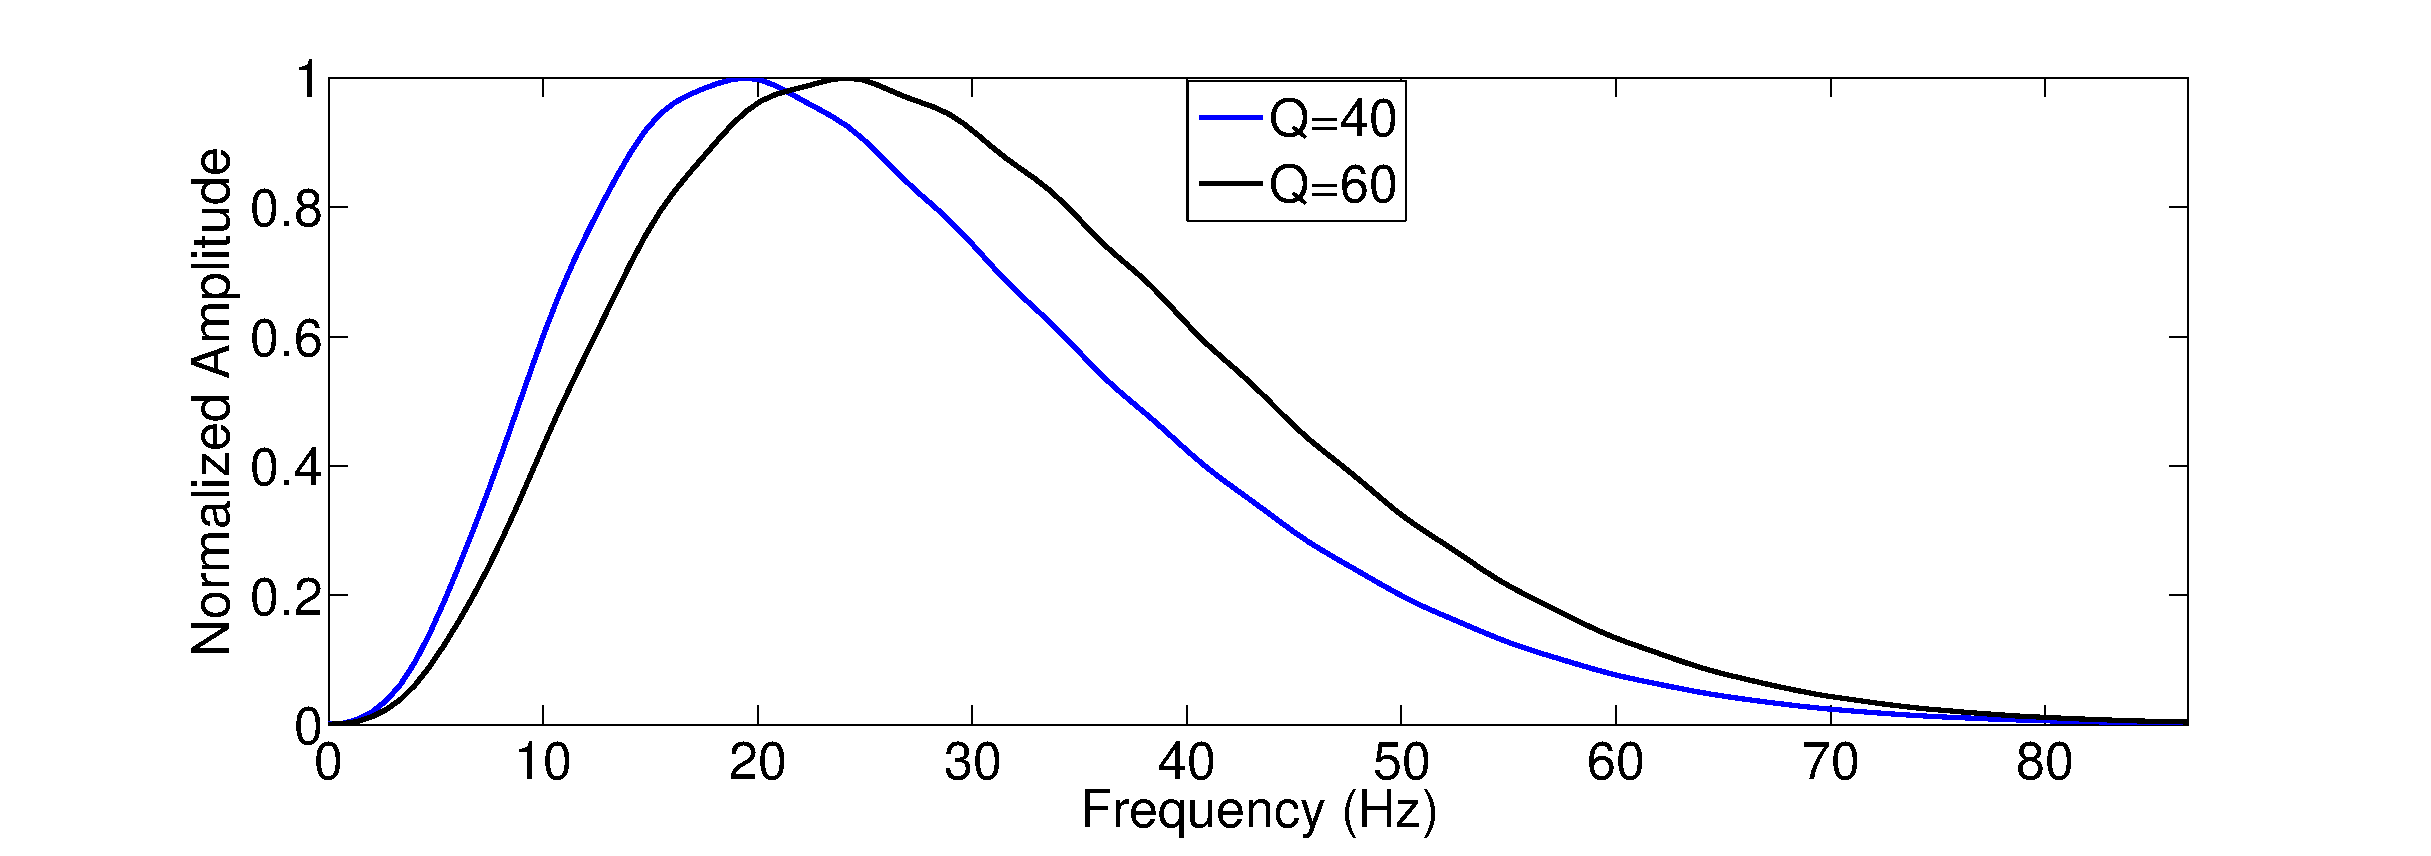
\includegraphics[width=0.92\linewidth]{figure/normalized_spectrum}}
    \fcaption{地震衰减效应:(a)不同$Q$值对地震波波形的影响;(b)不同$Q$值对地震波
	振幅谱的影响;(c)归一化的振幅谱。}{The effects of seismic attenuation:
    (a) the seismic waveforms propagated in different $Q$ models; (b) the amplitude 
	spectrum; (c) the nomalized amplitude spectrum.}
    [地震衰减效应]
    \label{fig:q_effect}
\end{figure*}
地震衰减不仅吸收地震波的振幅而且对地震波的相位有很强的改造作用(图~\ref{fig:q_effect}a)。
由第二章的线性粘弹理论知道,衰减系数$\alpha$与地震波的频率$f$成线性关系
(公式~\ref{eq:linear_visco}),即$\alpha\propto f$。
衰减介质对地震波高频成分的衰减要强于对低频成分的衰减(图~\ref{fig:q_effect}b),
这就导致了衰减介质中地震波的峰值频率往低频率处移动(图~\ref{fig:q_effect}c)。
几何扩散、透射损失等地震现象影响地震波的振幅但不影响地震波的峰值频率,
地震波峰值频率的大小基本只与地下介质衰减强度有关。\citeB{quan.harris:1997}
首次将模拟数据与观测数据间的质心频率差异作为匹配准则,用射线层析方程来更新
$Q$模型。为了克服射线理论高频近似的局限性,\citeB{dutta.schuster:2016}将峰值
频率移动目标函数引入到了波动层析当中,通过连接函数首次推导了压力波场对
驰豫参数$\tau(\mathbf{x})$的Frechet导数。同时也用伴随状态法推导出了峰值移动目标
函数对模型参数$\tau(\mathbf{x})$的梯度并给出了伴随源。他们的方法在理论合成数据
和实际数据中都获得了很好的效果,但是\citeB{dutta.schuster:2016}的$Q$层析方法
只用了直达波数据。

\begin{figure*}[!htbp]
    \centering
    {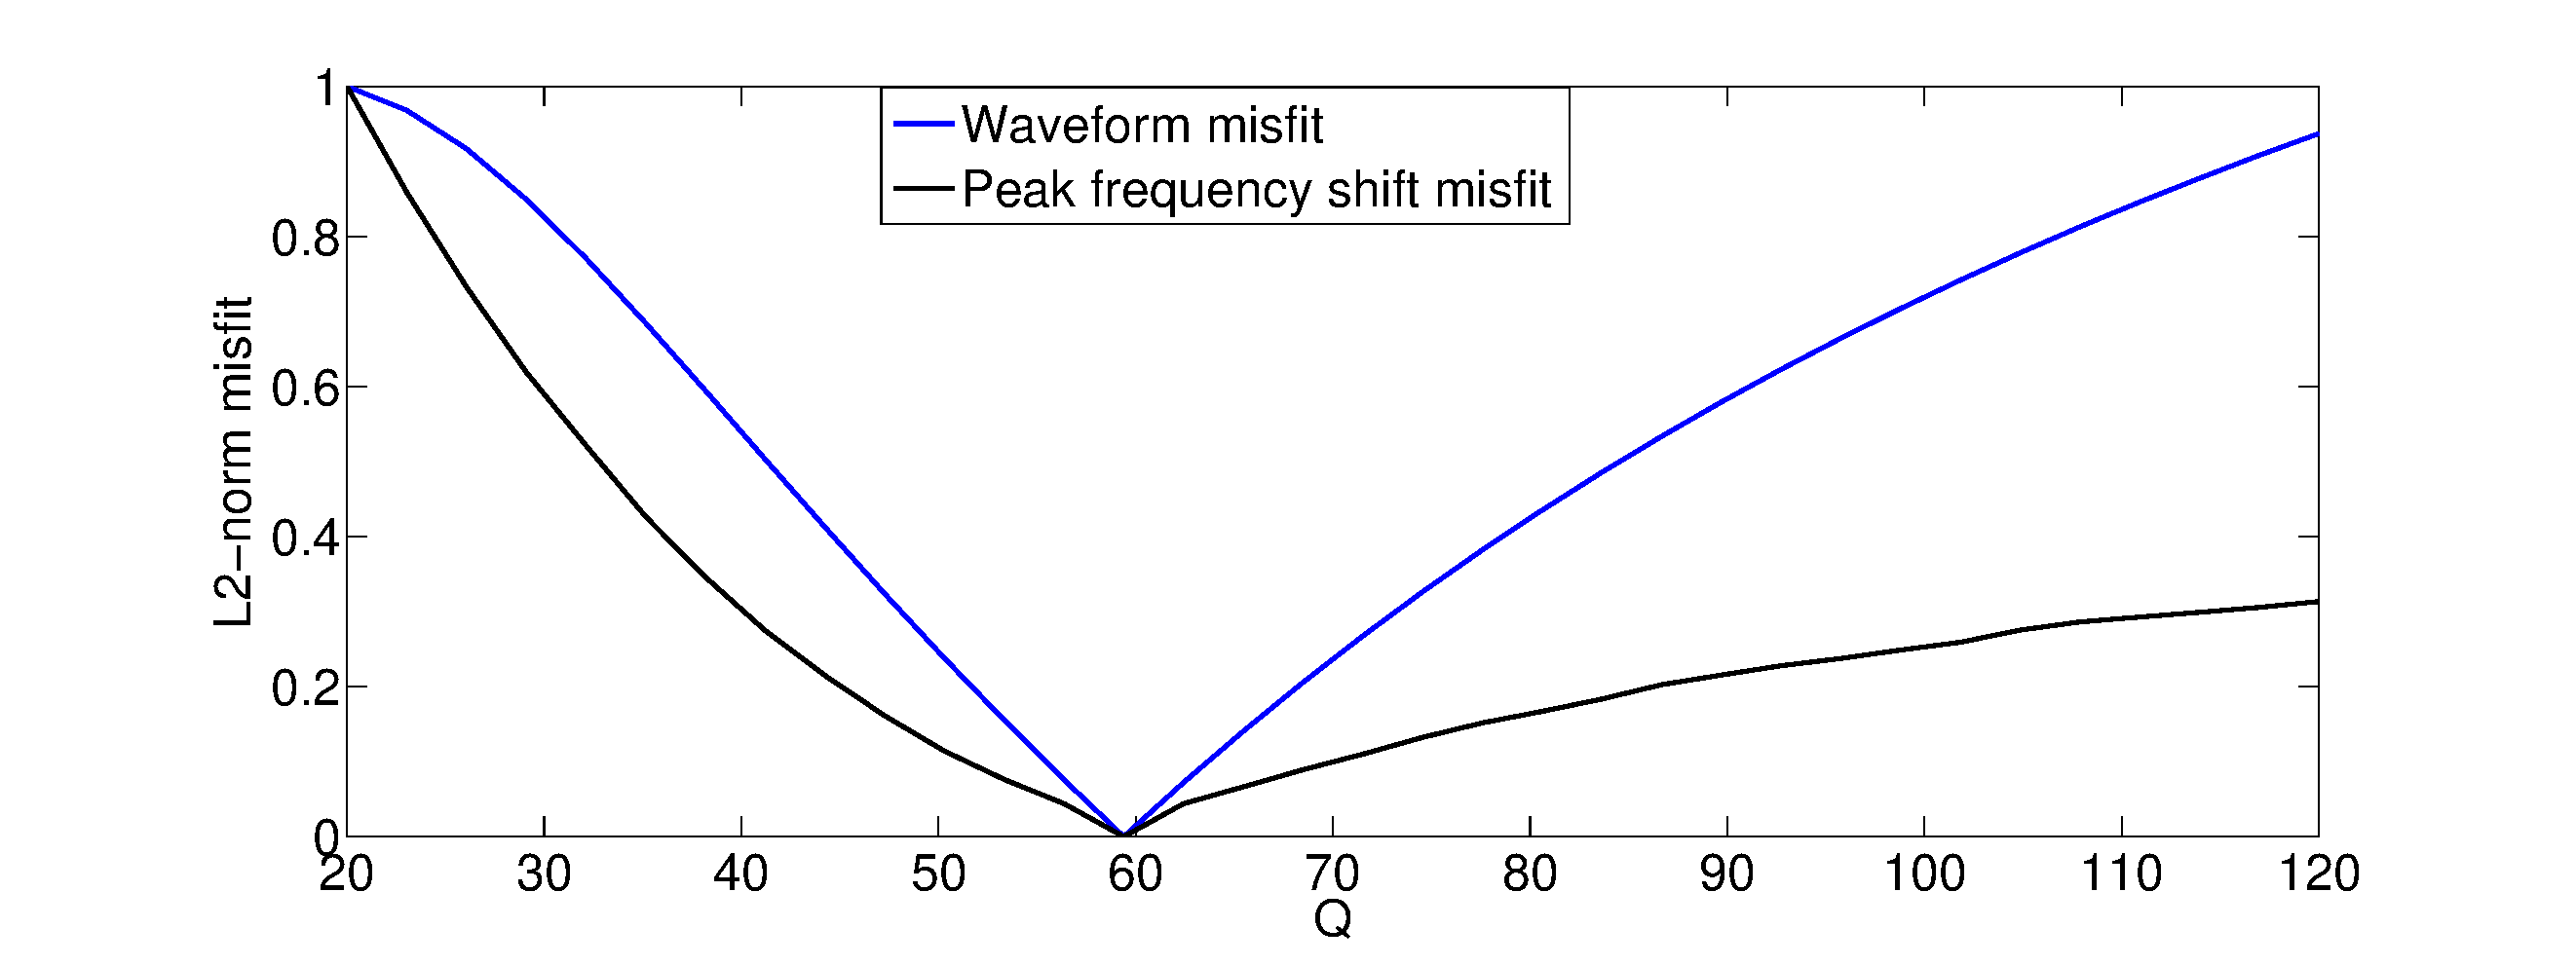
\includegraphics[width=0.92\linewidth]{figure/misfit_com}}
    \fcaption{两类归一化的目标函数随$Q$变化的形态,蓝线表示数据残差匹配最小二乘目
	标泛函,黑线表示峰值频率移动最小二乘目标泛函。}
	{Two types of misfit function vary with $Q$, blue line represents the least 
	squre of amplitue residual, and the black line represents the least squre of 
	the frequency shift.}[两类归一化的目标函数随$Q$变化的形态]
    \label{fig:misfit_com}
\end{figure*}
正如第三章所讲,相较于透射波,反射波能提供更深部的介质参数信息。
相比于振幅匹配的目标函数(公式~\ref{eq:misfit_function}),峰值频率移动的
目标函数具有如下表达式:
\begin{equation}
    \mathcal{J}(\mathbf{m})=\frac{1}{2}\sum_{s,g}\int_t\Delta f^2(\mathbf{x}_s,\mathbf{x}_g,t)dt,
    \label{eq:freq_misfit_function}
\end{equation}
其中$\Delta f(\mathbf{x}_s,\mathbf{x}_g,t)=f^{peak}_{obs}(\mathbf{x}_s,\mathbf{x}_g,t)-
f^{peak}_{cal}(\mathbf{x}_s,\mathbf{x}_g,t)$,$f^{peak}_{obs}(\mathbf{x}_s,\mathbf{x}_g,t)$
和$f^{peak}_{cal}(\mathbf{x}_s,\mathbf{x}_g,t)$分别是观测数据与模拟数据各震相的峰值
频率。图~\ref{fig:misfit_com}~展示了两种目标函数随$Q$值变化的形态。从图中可以看出
峰值频率移动的目标函数比波形残差目标函数具有更宽的收敛盆,更加适合背景$Q$模型的反演。
另外,将峰值频率移动作为匹配准则引入$Q$-RWI中可以降低反演方法对高波数速度模型的依赖。
反射波数据不同于直达波数据,通常具有多个震相。如何把反射波数据中各个震相的
峰值频率提取出来是反演成功的关键。本章先介绍基于峰值频率移动目标函数的
$Q$-RWI基本理论;然后给出提取多震相反射地震数据各个震相峰值频率的办法;
最后通过数值实验来证明所提反演方法的可靠性。


\vspace{1.5cm}
\section{方法原理}
\vspace{0.5cm}
基于峰值频率移动目标函数的$Q$-RWI算法步骤跟波动方程走时反演(\citeA{luo.schuster:1991};
\citeA{ma.hale:2013})类似。首先需要定义一个链接函数来连接峰值频率移动残差与声压波场的
关系;其次需要定义与峰值频率移动相关的目标泛函;最后需要用粘声波方程以及链接函数来推导
目标函数对$Q$的一阶导数即梯度方向。在这一章的推导中,我们假定地震波传播满足二维时间域
SLS模型粘声波方程~\ref{eq:state}。

用$\hat{P}_f(\mathbf{x}_s,\mathbf{x}_g,t)$表示给定背景$Q$模型的模拟震相,下标$f$表示
该震相的峰值频率,峰值频率从震相的振幅谱(图~\ref{fig:q_effect}c~中黑线)中获取。
类似地,用$P_{f-f_1}(\mathbf{x}_s,\mathbf{x}_g,t)$表示同一震相峰值频率为$f-f_1$的
观测数据,其震相的振幅谱用图~\ref{fig:q_effect}c~中的蓝线表示。其中,$f_1$表示由于
$Q$不准引起的模拟数据与观测数据间峰值频率的移动,为了方便表达,这一节我们假设地震数据中
只含有单一震相,多震相的峰值频率提取方法将在下一节中给出。

给定一个足够准确的背景速度模型,模拟数据与观测数据之间相似性可以定义为:
\begin{equation}
	F_{f_1}(\mathbf{x}_s,\mathbf{x}_g,t)=\int dt P_{f-f_1}(\mathbf{x}_s,\mathbf{x}_g,t) 
	\hat{P}_f(\mathbf{x}_s,\mathbf{x}_g,t).
	\label{eq:correlation}
\end{equation}
在这一章的$Q$-RWI算法中,主要是寻求最小的峰值频率移动。对于准确的背景$Q$模型,
观测数据和模拟数据具有相同的峰值频率。换句话说,就是寻求一个移动值$f_1=\Delta f$,
使其最大化方程~\ref{eq:correlation}中的互相关函数。如果$\Delta f=0$,表明我们找到了
正确的背景$Q$模型。

因为$f_1=\Delta f$最大化了互相关函数~\ref{eq:correlation},所以$F_{f_1}(\mathbf{x}_s,
\mathbf{x}_g,t)$对$f_1$的导数在$f_1=\Delta f$处为零,即:
\begin{equation}
	\begin{aligned}
		\dot{F}_{\Delta f}(\Delta f,\tau(\mathbf{x})) &=\left[\frac{\partial F_{f_1}
	(\mathbf{x}_s,\mathbf{x}_g,t)}{\partial f_1}\right]_{f_1=\Delta f}, \\
		&= \int dt \dot{P}_{f-\Delta f}(\mathbf{x}_s,\mathbf{x}_g,t)
	\hat{P}_f(\mathbf{x}_s,\mathbf{x}_g,t)=0,
	\label{eq:connective}
	\end{aligned}
\end{equation}
式中$\dot{F}_{\Delta f}(\Delta f,\tau(\mathbf{x}))=[\partial P_{f-f_1}(\mathbf{x}_s,
\mathbf{x}_g,t)/\partial f_1]_{f_1=\Delta f}$。方程~\ref{eq:connective}~即为链接函数,
链接函数作为一个中间方程来连接基础数据(声压波场)与骨架数据(频率移动残差)。因为波动方程
不能直接建立起骨架数据与模型参数的关系,所以在推导梯度时链接函数是必需的。

本章中,目标函数的定义如~\ref{eq:freq_misfit_function}~式。其梯度$\gamma(\mathbf{x})$
表示如下:
\begin{equation}
	\gamma(\mathbf{x})=\frac{\partial\mathcal{J}}{\partial \tau(\mathbf{x})}
	=-\sum_{s,g}\frac{\partial \Delta f}{\partial \tau(\mathbf{x})}
	\Delta f(\mathbf{x}_s,\mathbf{x}_g,t).
\end{equation}
从方程~\ref{eq:connective}~出发,可以得到如下三个方程:
\begin{equation}
	\begin{aligned}
		 &\dot{F}_{\Delta f}(\Delta f,\tau(\mathbf{x}))=0, \\
		&\Rightarrow \frac{\partial \dot{F}_{\Delta f}}{\partial \Delta f} 
		\frac{\partial \Delta f}{\partial \tau(\mathbf{x})} + 
		\frac{\partial \dot{F}_{\Delta f}}{\partial\tau(\mathbf{x})} =0, \\
		&\Rightarrow \frac{\partial \Delta f}{\partial \tau(\mathbf{x})} =
		-\frac{\frac{\partial \dot{F}_{\Delta f}}{\partial\tau(\mathbf{x})}}
		{\frac{\partial \dot{F}_{\Delta f}}{\partial \Delta f}},
	\end{aligned}
\end{equation}


\vspace{0.5cm}
\section{多震相反射数据峰值频率提取}
\section{数值实验}

